\section{Technique}
%
To add path merging to SPF, we first pre-compute static summaries of arbitrary code regions with more than one execution
path and methods.
%
To bound the set of code regions we analyze, we start by specifying a method $M$ in a configuration file.
%
Next, we construct a set containing only the class $C$ that contains $M$.
%
We then get another set of classes, $C'$,
such that every class in $C'$ has atleast one method that was called by a method in a class in $C$.
%
This step which goes from $C$ to $C'$ discovers all the classes at a call depth of 1 from $C$.
%
We continue this method discovery process up to a call depth of 2.
%
While we can increase the call depth in our method discovery process, we found that summarizing
arbitrary code regions more than 2 calls deep did not lead to practically useful region summaries.
%
After obtaining a list of methods, we computed static summaries of regions in these methods and method summaries as
explained in Section \ref{sec:static-analysis}.
%
To make use of region summaries in Symbolic PathFinder, we use an existing feature of SPF named \textit{listener}.
%
A listener is a method defined within SPF that is called for every bytecode instruction executed by SPF.
%
Java Ranger adds a path merging listener to SPF that, on every instruction, checks (1) if the instruction involves
checking a symbolic condition, and (2) if Java Ranger has a pre-computed static summary that begins at that
instruction\rq s bytecode offset.
%
If both of these conditions are satisfied, Java Ranger instantiates the multi-path region summary by reading inputs from
and writing outputs to the stack and the heap.
%
It then conjuncts the instantiated region summary with the path condition and resumes symbolic execution at the
bytecode offset of the end of the region.
%
The instantiation of the region summary is performed as a sequence of transformations described below and summarized
in Figure~\ref{fig:overview}.
%
\begin{figure}[]
    \caption{Overview of transformations on Ranger IR to create and instantiate multi-path region summaries with higher-order regions}
    \label{fig:overview}
    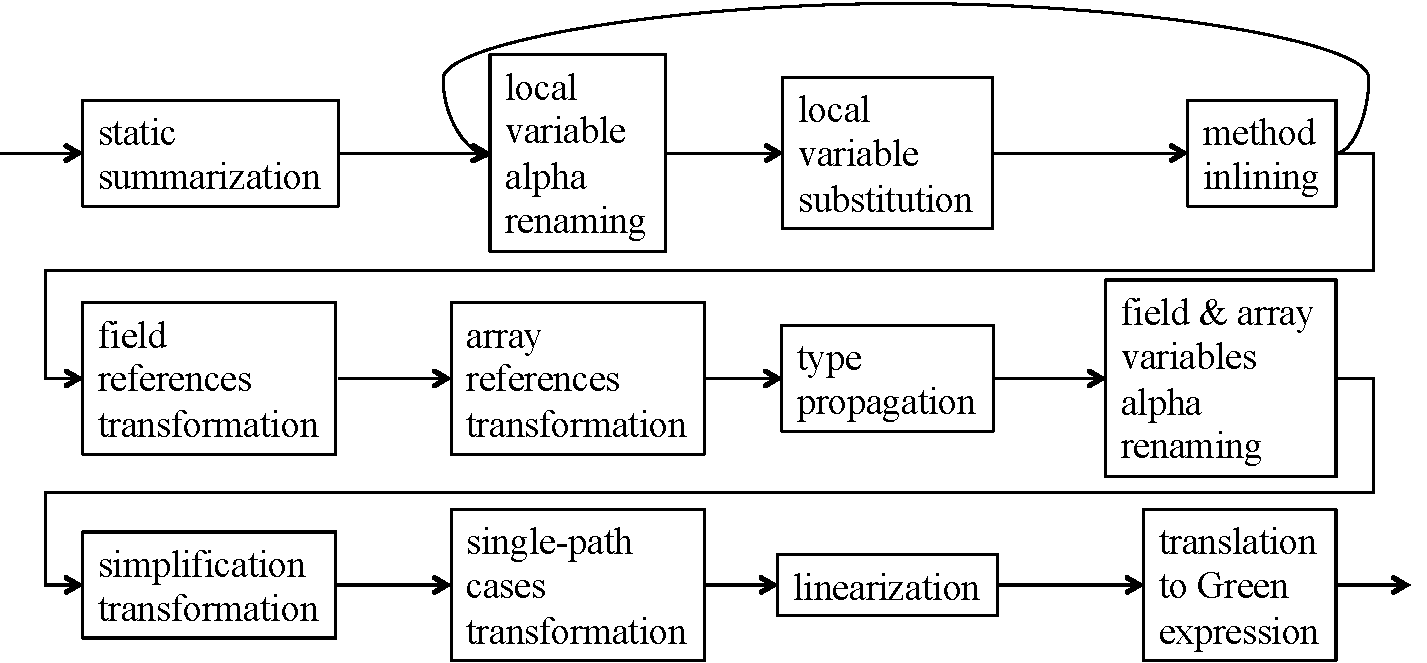
\includegraphics[width=\textwidth]{figures/overview.pdf}
\end{figure}
%
%
%\subsection{WALA-based analysis for veritesting}
%%
%Veritesting requires static construction of
%predicates of a multi-path region which represent changes to the path expression of the dynamic
%symbolic executor.
%%
%It also requires construction of a control-flow graph of method bodies
%from Java bytecode and finding exit points of the region, which in turn
%requires creation of a control-flow graph of the region.
%%
%Implementing veritesting is made simpler by using a static single
%assignment~(SSA)~\cite{ssa} representation of the multi-path region.
%%
%Using an SSA form allows us to use the $\phi$-expressions created by the
%SSA form and translate them into points at the end of the veritesting
%region where updates to system state along different paths in the region
%can be merged.
%%
%\mike{MWW: Vaibhav please update to describe WALA}
%WALA~\cite{} is a static analysis framework for Java programs that
%has both these features, with
%ExceptionalUnitGraph~\cite{exceptionalunitgraph} and the Shimple
%IR~\cite{shimple}.
%%
%For simple regions with only one exit point, like the one presented in Listing~\ref{lst:v_ex}, we
%were able to use Soot to automate static construction of the predicate representing
%an update to the expression.
%%
%For doing this, we used nodes with more than one successor as the
%starting point, found the immediate post-dominator of the starting
%point, and traversed the control-flow graph on all sides of such branches.
%%
%During such a traversal, we constructed predicates representing the
%multi-path region, similar to the ones presented in
%Listing~\ref{lst:v_ex_smt2}.
%%
%As explained in Section~\ref{sec:exit_points}, including virtual
%function invocations in the construction of our predicates amplifies the
%benefits of veritesting even further.
%%
%We plan to automate this inclusion in the future using Soot.
%%
%Providing SPF with updates to be made to its symbolic store also
%requires Soot to maintain stack location information for variables.
%%
%We plan to automate SPF\rq s symbolic store updates using Soot in the
%future.
%%
%

\subsection{Representation of Static Regions}
\label{sec:static-analysis}
\vaibhav{assigned to Mike}
\mike{MWW: - we should provide an AST of the constraint language}

\subsection{Instantiation-time Transformations}
\textbf{Alpha Renaming}: \vaibhav{assigned to Soha}\\
\textbf{Local Variable Substitution}: \vaibhav{assigned to Soha}\\
\textbf{Higher-order Regions}: \vaibhav{assigned to Soha}\\
\textbf{Field References SSA form}: The field references transformation translates reads and writes of fields
in Java bytecode into corresponding Ranger IR statements.
%
In order to translate all field accesses to SSA form, this transformation creates a summary of the semantics
represented by the field accesses in the region.
%
This transformation constructs a new field access variable for every field assignment on every path within the region.
%
This new field access variable construction makes use of two monotonically increasing subscripts.
%
It uses a path subscript to distinguish between assignments to the same field on the same execution path.
%
It uses a global subscript to distinguish between assignments to the same field across execution paths.
%
At the merge point of the region, field assignments done on the same field are merged using
Gated Single Assignment (GSA)~\cite{Ottenstein1990}.
%
Each merged field access variable has its own path and global subscripts and represents the output of the region into
its field.
%
The path subscript helps us resolve read-after-write operations on the same execution path and find the latest write
into a field on an execution path.
%
The global subscript helps us distinguish between field accesses across multiple execution paths. \\
\textbf{Array References SSA form}: The array references transformation translates reads and writes of arrays in
Java bytecode into corresponding Ranger IR statements.
%
In order to translate all array accesses to SSA form, this transformation creates an execution path-specific copy of
every array when it is first accessed within a region.
%
Reads and writes of arrays are then done on a path-specific copy of the array.
%
All array copies are merged at the merge point of multi-path regions.
%
The merged array copy represents array outputs of the region.\\
\textbf{Simplification of Ranger IR}: The Ranger IR constructed by earlier transformations computes exact semantics
of all possible behaviors in the region.
%
Representation of such semantics as a formula can often lead to unnecessarily large formulas, which has the potential to
reduce the benefits seen from path merging~\cite{angr}.
%
For example, if an entry in an array is never written to inside a region, the array reference transformation can still have an
array output for that entry that writes a new symbolic variable into it.
%
The region summary would then need to have an additional constraint that makes the new symbolic variable equal the
original value in that array entry.
%
Such conjuncts in the region summary can be easily eliminated with constant propagation, copy propagation, and constant
folding~\cite{dragon-book}.
%
Ranger IR also has statement and expression classes that use a predicate for choosing between two statements (similar to
an {\tt if} statement in Java) and two sub-expressions (similar to the C ternary operator) respectively.
%
When both choices are syntactically equal, the predicated statement and expression objects can be substituted with the
statement or expression on one of their two choices.
%
Such statements and expressions were simplified away to use one of their two choices.
%
Ranger IR performs these two simplifications on such predicated statements and expressions along with constant folding,
constant propagation, and copy propagation.\\
\textbf{Single Path Cases}: \vaibhav{assigned to Soha}\\
\textbf{Linearization}: \vaibhav{Soha, Mike, please feel free to rewrite.}
Ranger IR contains translation of branches in the Java bytecode to if-then-else statements defined in the Ranger IR.
%
But the if-then-else statement structure needs to be kept only as long as we have more GSA expressions to be
introduced in the Ranger IR.
%
Once all GSA expressions have been computed, the Ranger IR need not have its if-then-else statements anymore.
%
In other words, the $\gamma$ functions introduced by GSA are a functional representation of branching, which is what lets us
capture the semantics of everything happening on both sides of the branch.
%
Since the linearization transformation is done after every field and array entry has been unaliased and converted to
GSA, dropping if-then-else statements from the Ranger IR representation of the region summary reduces redundancy in its
semantics and converts it into a stream of GSA and SSA statements.\\
\textbf{Translation to Green}: \vaibhav{assigned to Soha}\\

\subsection{Checking Correctness Of Region Summaries}
The Ranger IR computed as a result of performing the transformations described in Figure~\ref{fig:overview} should
correctly represent the semantics of the summarized region.
%
If it doesn't, then using the instantiated region summary can cause symbolic exploration to explore the wrong behavior
of the subject program.
%
We checked the correctness of our instantiated region summaries by using equivalence-checking as defined by Ramos et al.~\cite{ramos}.
%
We designed a test harness that first executes the subject program with a set of symbolic inputs using SPF and
capture the outputs of the subject program.
%
Next, the test harness executes the same subject program with the same set of symbolic inputs using Java Ranger and
capture the outputs of the subject program once again.
%
Finally, the test harness compares outputs returned by symbolic execution with SPF and Java Ranger.
%
If the outputs do not match, then a region summary used by Java Ranger did not contain all the semantics
of the region it summarized.
%
We symbolically execute all execution paths through this test harness.
%
If no mismatch is found between outputs on any execution path, we conclude that all region summaries used by Java Ranger
must correctly represent the semantics of the regions they summarized.
%
We performed correctness-checking on all results reported in this paper.
